\documentclass[conference]{IEEEtran}
\usepackage{pifont}
\usepackage{times,amsmath,color,
amssymb,graphicx,epsfig,cite,psfrag,subfigure,algorithm,multirow,cases,balance}
\newtheorem{claim}{Claim}
\newtheorem{guess}{Conjecture}
\newtheorem{definition}{Definition}
\newtheorem{fact}{Fact}
\newtheorem{assumption}{Assumption}
\newtheorem{theorem}{\underline{Theorem}}
\newtheorem{lemma}{\underline{Lemma}}
\newtheorem{ctheorem}{Corrected Theorem}
\newtheorem{corollary}{\underline{Corollary}}
\newtheorem{proposition}{Proposition}
\newtheorem{example}{\underline{Example}}
\newtheorem{remark}{\underline{Remark}}
\newtheorem{problem}{\underline{Problem}}
\def\Ei{\mathop\mathrm{Ei}}
\def\E{\mathop\mathrm{E}}
\def\tr{\mathop\mathrm{tr}}
\newcounter{mytempeqncnt}
%\IEEEoverridecommandlockouts

\begin{document}

\title{Literature Survey -- Draft II \\ Unsupervised Feature Learning and Deep Learning}
\author{Jiachen Li (Andrew ID: jiachenl)\\%
Language Technologies Institute, Carnegie Mellon University, Pittsburgh, PA, 15213, USA\\
Email: jiachenl@cs.cmu.edu
}

%\thanks{This work was supported...}




\maketitle %\thispagestyle{empty}




\begin{abstract}
Machine Learning has proven to be a big success in many areas of artificial intelligence. However, the success of these algorithms highly depends on how good the features are represented. A good representation of feature is surely
to enhance the performance of machine learning algorithms, while a poor representation may not only severely limit the performance
but even ruin the results. In this literature survey, I will do a review about the field of unsupervised feature learning and has an emphasis on learning feature representation through deep learning architecture. This survey will start with the problems about unsupervised feature learning. After that, it will introduce some typical algorithms in unsupervised feature learning and deep learning. Moreover, it will provide a few successful examples by using unsupervised feature learning. Finally, the conclusion as well as the potential feature works will be included at last.

\end{abstract}

\section{Introduction}

The performance of machine learning algorithms, especially the simpler ones  highly depends on how good the features are represented \cite{review}. For this reason, much of the effort in deploying machine learning algorithms in real problems has been paid to the process of feature extraction. During the past decades, feature extraction does play an very important role in the development of machine learning, where the machine learning research communities have spent a lot of efforts on manually designing or creating new features through domain knowledge and some other special techniques. For example, the MFCC feature in speech recognition and the HoG feature in computer vision. However, though these features may often contain the deep insights about a specific problem or some incredibly clever ideas, we cannot avoid the fact that the way to create such features costs a lot of human labor and the feature representation derived often cannot be extended to other problems, especially when we encounter into them in a new filed. So the problem comes up that is there any way to learn the feature representation automatically and is there any way to do better than the manually created features. Fortunately, the answer is yes to both of the questions, and the way is unsupervised feature learning.

\subsection{What Is Unsupervised Feature Learning?}

\begin{figure}[t]
\centering
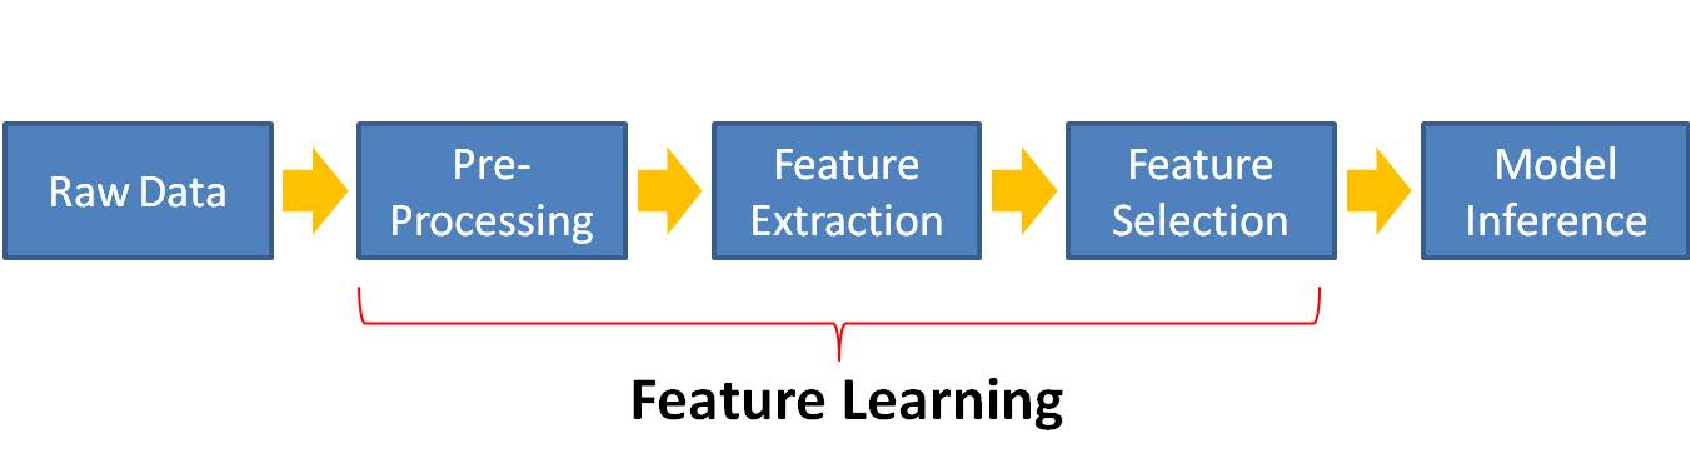
\includegraphics[width=90mm]{feature_learning.pdf}
\caption{The general framework of machine learning task.}
\label{fig:ml_task}
\end{figure}

To answer the question that what is unsupervised feature learning, let's start by looking at the general framework of solving a machine learning task. To solve a machine learning problem, as shown in Fig. \ref{fig:ml_task}, we should first do pre-precessing for the raw data, such as the data cleaning, and then perform feature extraction on the data processed. After that, we apply our feature extraction algorithm to extract the useful features, do feature selection on these extracted features and then use them for training models. With a well trained model, we can finally approach to our goals like classification or regression.

In the above framework, the procedures of pre-processing, feature extraction and feature selection together can be summarized as the ``feature learning''. 
Moreover, the term ``unsupervised'' means that we can this kind of feature learning procedures to be performed without our supervision (knowledge) or even without any of our help.

\subsection{Differences with other Machine Learning Tasks}



One of the major differences that distinguishes unsupervised feature learning from other machine learning tasks such as classification is the ultimate goal during the training phase. To be specific, in the case of classification, the typical objective is to minimize the classification errors on the training set, so that we can learn a classifier or predictor for future use. However, in the unsupervised feature learning, the goal changes to learn the representation of feature automatically, which means the algorithms will make their own decisions on what is going to learn. Therefore, the features learned will no long be specified by human. And this is also totally different from the paradigm of feature engineering where people design by hands on what to learn.

\subsection{Types of Unsupervised Feature Learning}

There are two common unsupervised feature learning settings, depending on what type of unlabeled data you have. The more general and powerful setting is the self-taught learning setting, which does not assume that your unlabeled data $\mathbf{x}_u$ has to be drawn from the same distribution as your labeled data $\mathbf{x}_l$ \cite{self_taught}. The more restrictive setting where the unlabeled data comes from exactly the same distribution as the labeled data is sometimes called the semi-supervised learning setting. This distinctions is best explained with an example, which we now give.

\subsection{Organization of this Review}

The reminder of this literature survey is organized as follows: Section II defines the feature learning problem and the learning strategy. Section III introduces the deep learning architecture. Section IV presents different learning algorithms while a few successful examples are then given in section V. Finally, the conclusion and potential future work are drawn in section VI.

\section{Feature Learning Problem and Learning Strategy}

Suppose that we have a large set labelled or unlabelled data as input, i.e., $$\mathcal{S}=\{\mathbf{x}^{(1)},\mathbf{x}^{(2)},\mathbf{x}^{(3)},\ldots\}, \ \mathbf{x}^{(i)}\in\mathcal{R}^n.$$
Then what the feature learning wants to do is to train a model 
\begin{equation}
\Psi(\mathbf{x}):\mathcal{X} \rightarrow \mathcal{F},
\end{equation}
which can extract rich and high-level structures (as the high-level features) from the origin input space ($\mathcal{X}$) to the feature space ($\mathcal{F}$). So the problem is how can we let the machine automatically learn such kinds of feature?

The answer to this question is to learn the feature by levels or layers, which means that to learn the final representation of the data, we may start by learning some lower level representation of the data (low level feature). Next, with the combination of these low level features, we can then further learn some higher level representation of the data (high level feature). So, if we continue this process, then we can finally learn a good representation of the data.

\begin{figure}[t]
\centering
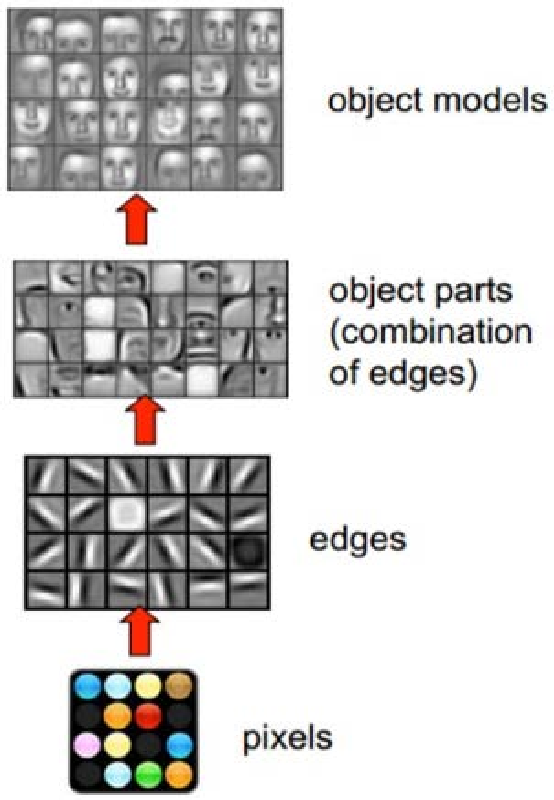
\includegraphics[width=65mm]{feat_level.pdf}
\caption{An illustration of learning feature representation by levels \cite{face}.}
\label{fig:feat_level}
\end{figure}


This layer-based learning strategy is first inspired by the study of our vision system, where the researchers reveal that information processing in our visual system has levels. For example, as shown in Fig. \ref{fig:feat_level}, if our visual system want to learn some representations of different faces with the pixel input from eyes, it may first try to learn the representation of edges (low level feature) from the input pixels. Then, with the combination of different edges, it can further learn the representation of different object parts on our faces, such as noises, mouses and so on (medium level feature). Finally, with the combination of these different object parts, we can learn to form different faces, which can be regarded as the high level feature.

\begin{remark}
The layer-based learning strate
\end{remark}

\section{Feature Learning Models: From Shallow to Deep}

\subsection{Background and Motivation}

Deep learning is a learning method where the deep architecture (e.g., multi-layer) is applied to perform the intellectual learning like learning to represent feature. This ability, together with the efficient learning algorithms that can ensure this ability, point out a new direction in the task of unsupervised feature learning, i.e., learning deep representation of the feature. In this section, I will review the work related to the deep learning in recent years, with respect to different types of architectures and learning algorithms. The application of it in unsupervised feature learning will be discussed in the next section.


\subsection{Type of Deep Neural Nets}

There are several types of deep neural nets, but deep belief networks and convolutional neural networks are two milestones in the realm of deep learning. Therefore, in this section, I'll mainly cover the details about these two types of deep learning architectures.

\subsubsection{Deep Belief Nets (DBNs)}


DBNs is a hybrid model consisting of two parts. As shown in Fig. \ref{fig:dbn}, the top two levels are undirected graph model which form the associative memory, the remaining layers are directed graph model which is actually a stacked Restricted Boltzmann Machines (RBM). Different from the CNNs, DBNs is a stochastically learning architecture whose object
function depends on the learning purpose. Generally speaking, DBNs can be trained as a discriminative model or a generative model. In Fig. \ref{fig:dbn} , the discriminative model is a ``bottoms-up'' approach (red arrow), trying to
learn the detection weights via optimizing a posterior probability $P(L|O)$, where $L$ indicates the label while $O$ is the observation; the generative model is a ``top-down'' approach (green arrow), trying to learn the generative weights via optimizing a joint probability $P(L,O)$. The details of the learning strategies will be discussed in the next part of this section.

The greatest advantage of DBNs is its capability of learning multi-level representation of feature, which is achieved through a layer-wise training strategy where the higher-level features are learned based on the features produced by the previous layers. Therefore, the higher-level features are believed to be more complicated and can better represent the information extracted from the structure of input data. Furthermore, we can also prove that after we adding another layer of features, we improve a variational lower bound on the log probability of the training data \cite{Hinton}.

\begin{figure}[t]
\centering
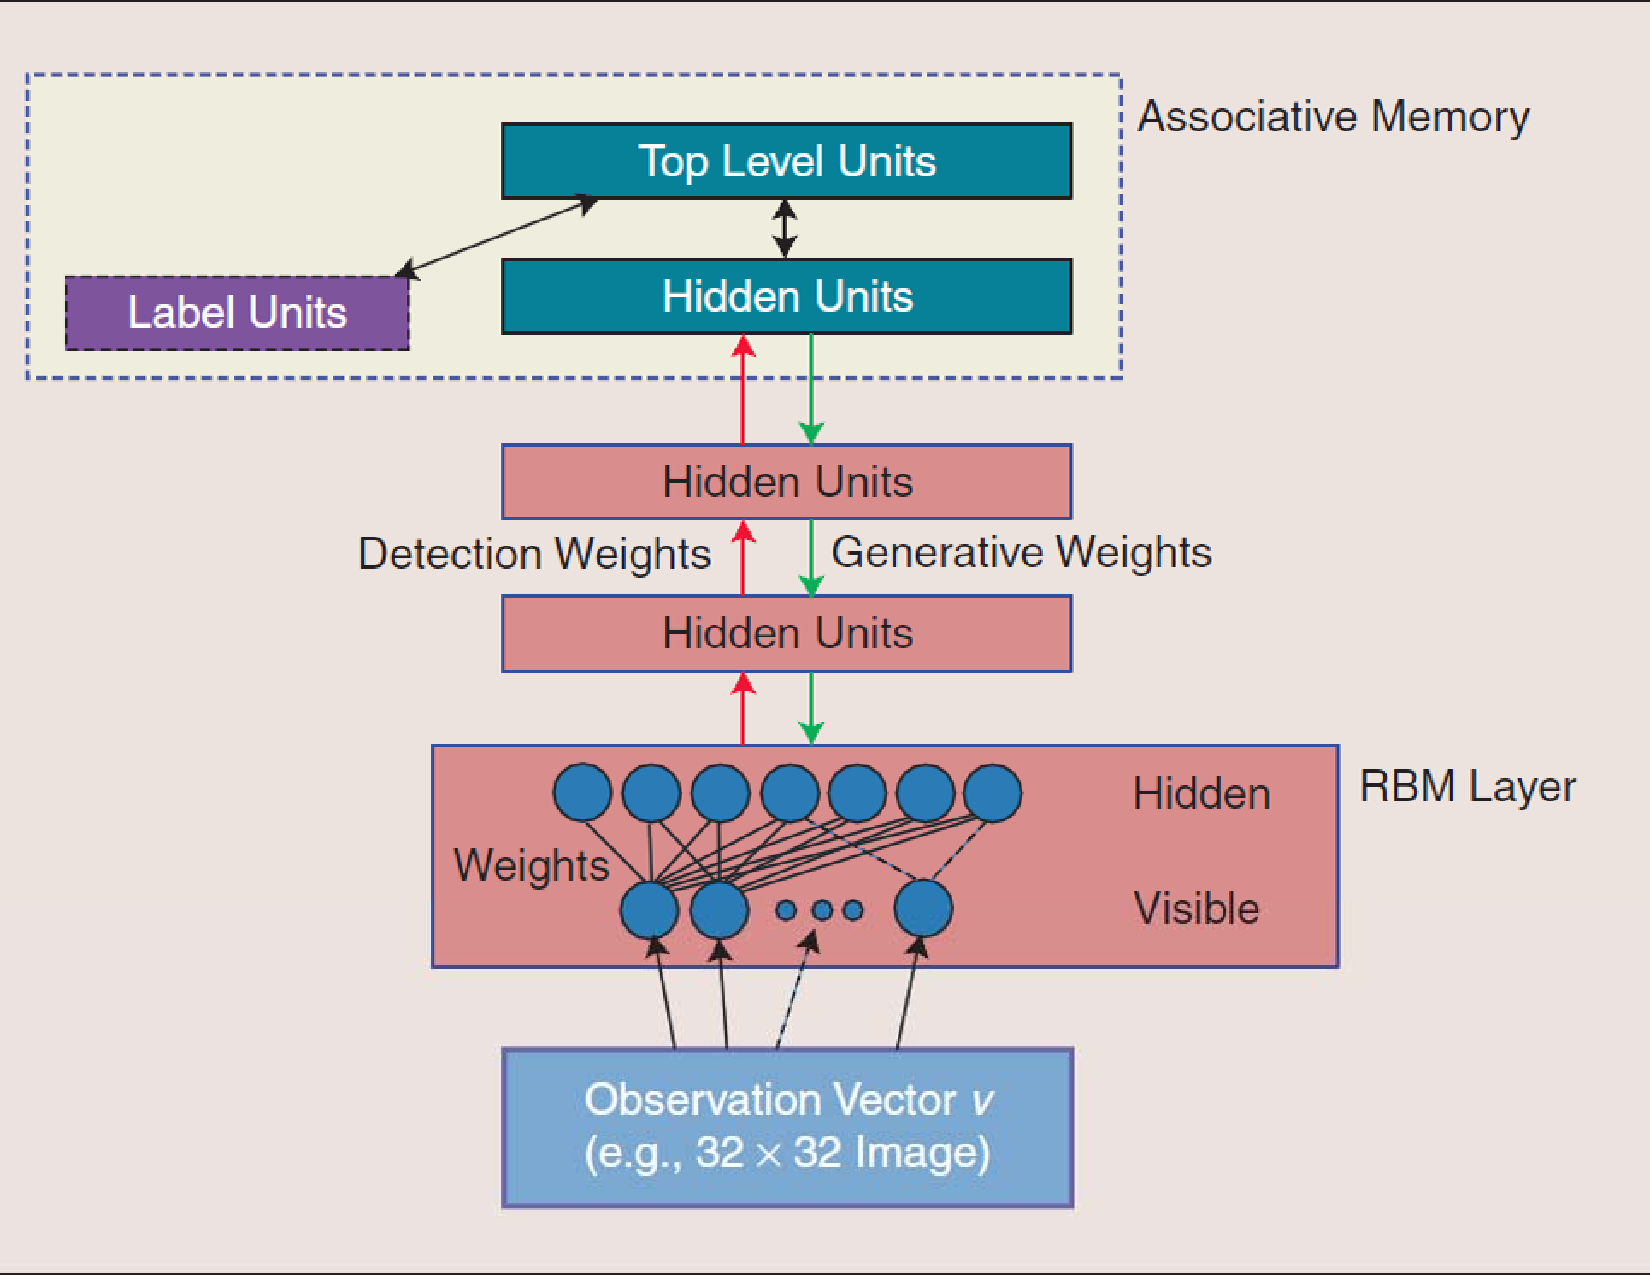
\includegraphics[width=75mm]{dbn.pdf}
\caption{Illustration of deep belief network framework\cite{new_frontier}.}
\label{fig:dbn}
\end{figure}

\subsubsection{Deep Convolutional Neural Nets (CNNs)}

TODO

\subsection{How to Train the Deep Neural Nets}

In this part, I'll discuss the training strategy in deep learning architecture. We will focus on the training of DBNs since it is not only one of the typical models in deep learning, but also very suitable for the feature learning.

Generally speaking, the training process of DBNs usually consists of two parts, one is the pre-training, the other is fine-tuning.

\subsubsection{Pre-Training}

In the part of pre-training, one of the popular and easy-implement choice is the greedy layer-wise unsupervised pre-training \cite{greedy}. The key idea of this approach is to learn a hierarchy of features one level at a time, using unsupervised feature learning to learn a new transformation at each level to be composed with the previously learned transformations. During the learning phase, each iteration of unsupervised feature learning adds a new layer of weights to the whole deep neural network. Finally the set of layers could be combined to transform the input data into a set of learned high-level features through a series of non-linear transformation.

TODO: another pre-training methods, RBM pre-training.

\subsubsection{Fine-tuning}

After pre-training, the weights between each adjacent layers can somehow reflect the relationship with the data themselves. Furthermore, in order to ensure a better performance, we use fine-tuning to adjust these weights according to different model types we assume.

For the generative model,...

For the discriminative model,...





\section{Unsupervised Feature Learning Algorithms}

In this section, I'll discuss in detail about several typical unsupervised feature learning algorithms. I'll not only cover the details about how them work, but also try to give explanations on why them work.


\subsection{Learning Feature Combination}

TODO

\subsection{Learning Feature Hierarchy}

TODO

\subsection{Another algorithm}

TODO

\section{Applications of Unsupervised Feature Learning}

In this section, I'll refer to some successful real world application to show the usage as well as the benefit of feature learning. The first example I'd like to show is the unsupervised feature learning in Image Recognition
And the second example I want to show is about the unsupervised feature learning in speech recognition.

\subsection{Unsupervised Feature Learning in Image Recognition}
TODO

\subsection{Unsupervised Feature Learning in Speech Recognition}
TODO





\begin{remark}
Sample remark...
\end{remark}


\section{Conclusions}

In this literature survey, ...

\section*{Acknowledgement}
I would like to thank...


%\balance
\begin{thebibliography}{99}

\bibitem{review} Y. Bengio, A. Courville, and P. Vincent, ``Representation Learning: A Review and New Perspectives,'' in \textit{IEEE Trans. Pattern Analysis and Machine Intelligence}, vol. 35, no. 8, pp. 1798--1828, 2013.

\bibitem{self_taught} R. Raina, A. Battle, H. Lee, B. Packer, and A. Y. Ng. ``Self-taught learning: Transfer learning from unlabeled data,'' \textit{Proc. Int'l Conf. Machine Learning}, 2007.

\bibitem{face} H. Lee, R. Grosse, R. Ranganath, and A. Y. Ng, ``Unsupervised Learning of Hierarchical Representations with Convolutional Deep Belief Networks'' \textit{Communications of the ACM}, vol. 54, no. 10, pp. 95--p103, 2011.


\bibitem{new_frontier} I. Arel, D. C. Rose, and T. P. Karnowski, ``Research frontier: Deep machine learning-a new frontier in artificial intelligence research,'' \textit{Comp. Intell. Mag.}, vol. 5, no. 4, pp. 13--18, Nov. 2010.

\bibitem{Hinton} G. E. Hinton, S. Osindero, and Y. Teh, ``A fast learning algorithm for deep belief nets,'' \textit{Neural Computation}, 18, pp 1527--1554, 2006.

\bibitem{greedy}  Y. Bengio, P. Lamblin, D. Popovici, and H. Larochelle, ``Greedy Layer-Wise Training of Deep Networks,'' \textit{Proc. Neural Information and Processing Systems}, 2006.

\bibitem{dAE} P. Vincent, H. Larochelle, Y. Bengio, and P. Manzagol. ``Extracting and composing robust features with denoising autoencoders,'' \textit{Proc. Int'l Conf. Machine Learning}, 2008.
\bibitem{CNN} H. Lee, R. Grosse, R. Ranganath, and A. Y. Ng, ``Convolutional deep belief networks for scalable unsupervised learning of hierarchical representations,'' \textit{Proc. Int'l Conf. Machine Learning}, 2009.
\bibitem{why} D. Erhan, Y. Bengio, A. Courville, P. Manzagol, P. Vincent, and S. Bengio, ``Why Does Unsupervised Pre-training Help Deep Learning?'' \textit{Journal of Machine Learning Research}, 2010.
\bibitem{kmeans} A. Coates and A. Y. Ng, ``Learning Feature Representations with K-means,'' \textit{Neural Networks: Tricks of the Trade}, Springer LNCS, 2012.

\bibitem{Yudong} L. Deng and D. Yu ``DEEP LEARNING: Methods and Applications,'' NOW Publishers, 2014.



\end{thebibliography}

\section{SUMMARY}

This is the first draft of my literature survey, I mainly finished: \\
1. The framework of the entire survey, i.e. what I shouldp cover in my literature survey. (Since the unsupervised feature learning is indeed not a very small area, so it really takes me some time to think it over on what should be included.) \\
2. The part of problem definition and background. \\
3. Part of the algorithm, i.e. the deep learning architecture. \\
4. Bibliography in full citation form. \\

For the next survey draft, I'm planning to finish: \\
1. The deep learning part. \\
2. The algorithm part. \\
3. One application example in the application part. \\
4. Include some theoretical analysis. \\
5. Polish the language usage.

%\begin{table}[t]\label{Tab:1}
%\centering \caption{$Required\ Interference\ Protection\
%Ratios$}
%\begin{tabular}{|c|c|c|}
%\hline
%Type of service & Channel & Interference \\
%& Offset & Protection D/U \\
%& & Ratio(dB) \\
%\hline
%Analog TV & Lower Adjacent & -14 \\
%\cline{2-3}
%& Co-channel & 34 \\
%\cline{2-3}
%& Upper Adjacent & -17 \\
%\hline
%Digital TV & Lower Adjacent & -28 \\
%\cline{2-3}
%& Co-channel & 23 \\
%\cline{2-3}
%& Upper Adjacent & -26 \\
%\hline
%\end{tabular}
%\end{table}








\end{document}
